\documentclass[twocolumn,traditabstract]{aa}  
\usepackage{fixltx2e}
\usepackage[english]{babel}
\usepackage{graphicx,amsmath}
%\usepackage{epstopdf}
\usepackage{epsf,color}
\usepackage[mathscr]{eucal}
\usepackage{amsmath}
\usepackage{amssymb,amsfonts}
\usepackage{natbib}
\usepackage{txfonts}
\usepackage{dsfont}
\definecolor{Mygreen}{rgb}{0.00, 0.72, 0.0}
\definecolor{Mypink}{rgb}{1.0, 0.0, 0.5}
\usepackage[breaklinks, citecolor=blue, linkcolor=Mygreen, urlcolor=Mypink, colorlinks=true, debug, baseurl=' ']{hyperref}
\usepackage{float}
\usepackage{color}
%\usepackage{scrextend}
%\usepackage{nccmath}
%\usepackage{mathtools, cuted}
%\usepackage{lscape}
\usepackage{widetext}
%\usepackage{flushend}
%\usepackage[T1]{fontenc}


\newcommand{\nika}{{\it NIKA}}
\newcommand{\nikad}{{\it NIKA2}}


\def\intk#1{\displaystyle\int\frac{d^2k_{#1}}{(2\pi)^2}}
\def\intr#1{\displaystyle\int d^2r_{#1}}
\def\simlt{\lower.5ex\hbox{$\; \buildrel < \over \sim \;$}}
\def\simgt{\lower.5ex\hbox{$\; \buildrel $\textgreater$ \over \sim \;$}}
\def\NIKA{\textit{NIKA}}
\def\NIKAd{\textit{NIKA2}}
\def\Archeops{\textit{Archeops}}
\def\Planck{\textit{Planck}}
\def\WMAP{\textit{WMAP}}
\def\Skydip{\textit{Skydip}}

\bibpunct{(}{)}{;}{a}{}{,}
\bibliographystyle{aa}

\begin{document}
\title{Polarization Spectral Energy Distribution of the Crab Nebula in prospect of future CMB experiments}
%\author{A.~Ritacco \inst{\ref{LPSC}}\thanks{Corresponding author: Alessia Ritacco, \url{ritacco@lpsc.in2p3.fr}}
\and  N.~Ponthieu \inst{\ref{IPAG}}
\and  A.~Catalano \inst{\ref{LPSC}}
\and R.~Adam \inst{\ref{LPSC},\ref{OCA}}
\and  P.~Ade \inst{\ref{Cardiff}}
\and  P.~Andr\'e \inst{\ref{CEA}}
\and  A.~Beelen \inst{\ref{IAS}}
\and  A.~Beno\^it \inst{\ref{Neel}}
\and  A.~Bideaud \inst{\ref{Neel}}
\and  N.~Billot \inst{\ref{IRAME}}
\and  O.~Bourrion \inst{\ref{LPSC}}
\and  M.~Calvo \inst{\ref{Neel}}
\and  G.~Coiffard \inst{\ref{IRAMF}}
\and  B.~Comis \inst{\ref{LPSC}}
\and  F.-X.~D\'esert \inst{\ref{IPAG}}
\and  S.~Doyle \inst{\ref{Cardiff}}
\and  J.~Goupy \inst{\ref{Neel}}
\and  C.~Kramer \inst{\ref{IRAME}}
\and  S.~Leclercq \inst{\ref{IRAMF}}
\and  J.F.~Mac\'ias-P\'erez \inst{\ref{LPSC}}
\and  P.~Mauskopf \inst{\ref{Cardiff},\ref{Arizona}}
\and A. Maury \inst{\ref{CEA}}
\and  F.~Mayet \inst{\ref{LPSC}}
\and  A.~Monfardini \inst{\ref{Neel}}
\and  F.~Pajot \inst{\ref{IAS}}
\and  E.~Pascale \inst{\ref{Cardiff}}
\and  L.~Perotto \inst{\ref{LPSC}}
\and  G.~Pisano \inst{\ref{Cardiff}}
\and M.~Rebolo-Iglesias  \inst{\ref{LPSC}}
\and  V.~Rev\'eret \inst{\ref{CEA}}
\and  L.~Rodriguez \inst{\ref{CEA}}
\and  C.~Romero \inst{\ref{IRAMF}}
\and F.~Ruppin \inst{\ref{LPSC}}
\and G.~Savini \inst{\ref{London_college}}
\and  K.~Schuster \inst{\ref{IRAMF}}
\and  A.~Sievers \inst{\ref{IRAME}}
\and C. Thum \inst{\ref{IRAME}}
\and  S.~Triqueneaux \inst{\ref{Neel}}
\and  C.~Tucker \inst{\ref{Cardiff}}
\and  R.~Zylka \inst{\ref{IRAMF}}}

%\institute{
Laboratoire de Physique Subatomique et de Cosmologie, Universit\'e Grenoble Alpes, CNRS/IN2P3, 53, avenue des Martyrs, Grenoble, France
  \label{LPSC}
  \and
  Laboratoire Lagrange, Universit\'e C\^ote d'Azur, Observatoire de la C\^ote d'Azur, CNRS, Blvd de l'Observatoire, CS 34229, 06304 Nice cedex 4, France
  \label{OCA}
  \and
Institut de RadioAstronomie Millim\'etrique (IRAM), Grenoble, France
  \label{IRAMF}
\and
Laboratoire AIM, CEA/IRFU, CNRS/INSU, Universit\'e Paris Diderot, CEA-Saclay, 91191 Gif-Sur-Yvette, France 
  \label{CEA}
\and
Astronomy Instrumentation Group, University of Cardiff, UK
  \label{Cardiff}
\and
Institut d'Astrophysique Spatiale (IAS), CNRS and Universit\'e Paris Sud, Orsay, France
  \label{IAS}
\and
Institut N\'eel, CNRS and Universit\'e Grenoble Alpes, France
  \label{Neel}
\and
Institut de RadioAstronomie Millim\'etrique (IRAM), Granada, Spain
  \label{IRAME}
\and
Dipartimento di Fisica, Sapienza Universit\`a di Roma, Piazzale Aldo Moro 5, I-00185 Roma, Italy
  \label{Roma}
\and
Univ. Grenoble Alpes, CNRS, IPAG, F-38000 Grenoble, France 
  \label{IPAG}
    \and
Aix Marseille Universit\'e, CNRS, LAM (Laboratoire d'Astrophysique de Marseille) UMR 7326, 13388, Marseille, France
  \label{LAM}
\and
School of Earth and Space Exploration and Department of Physics, Arizona State University, Tempe, AZ 85287
  \label{Arizona}
\and
Universit\'e de Toulouse, UPS-OMP, Institut de Recherche en Astrophysique et Plan\'etologie (IRAP), Toulouse, France
  \label{IRAP}
\and
CNRS, IRAP, 9 Av. colonel Roche, BP 44346, F-31028 Toulouse cedex 4, France 
  \label{IRAP2}
\and
University College London, Department of Physics and Astronomy, Gower Street, London WC1E 6BT, UK
  \label{UCL}
\and 
Institut d'Astrophysique de Paris, CNRS (UMR7095), 98 bis boulevard Arago, F-75014, Paris, France
  \label{IAP}
\and 
LERMA, CNRS, Observatoire de Paris, 61 avenue de l'Observatoire, Paris, France
  \label{LERMA}
}

\date{Received \today \ / Accepted --}
	
\abstract{The detection of the primordial B-modes constitutes one of the major challenges of modern cosmology. The precise measurement of this signal requires an accurate determination of foreground contaminants and of the absolute calibration of the instrument in terms of cross polarization and absolute polarization angle reconstruction.  We  present here a study of the Crab nebula, which is a well known polarization angle calibration source. The Crab nebula represents the most intense source in the microwave sky with an extension of few arcminutes corresponding to the typical beam of current CMB experiments. The Crab nebula exhibits a highly polarized synchrotron radiation at radio and millimeter wavelengths.
In this paper we present Crab Stokes $I$, $Q$ and $U$ maps obtained at 150 GHz with the \NIKA\ camera. 
\NIKA\ has been operated at IRAM 30 m telescope from 2012 to 2015. It is a camera made of Lumped Element Kinetic Inductance Detectors (LEKIDs) and observing the sky at 150 and 260 GHz. 
We report in this paper high resolution (18$^{\prime\prime}$) FWHM observations of the Crab nebula in intensity and polarization at 150 GHz. From the observations we are able to reconstruct the spatial distribution of polarization degree and angle, which is found to be compatible with previous observations at lower and higher frequencies. Averaging across the source we measure the polarization angle of the Crab nebula at arcmin scales to better than \%. Using previous observations we also present the first estimation of the Spectral Energy Distribution in polarization.  These measurements will be of interest for current and next generation of CMB experiments operating at (sub)-mm wavelengths. }
\titlerunning{Polarization SED of the Crab nebula}	
\authorrunning{A. Ritacco, J. F. Mac\'ias P\'erez , N. Ponthieu et al.}
\keywords{Techniques: polarization -- KIDs --  individual: NIKA }
\maketitle
\begin{figure*}[h!]
  \centering
     	  { 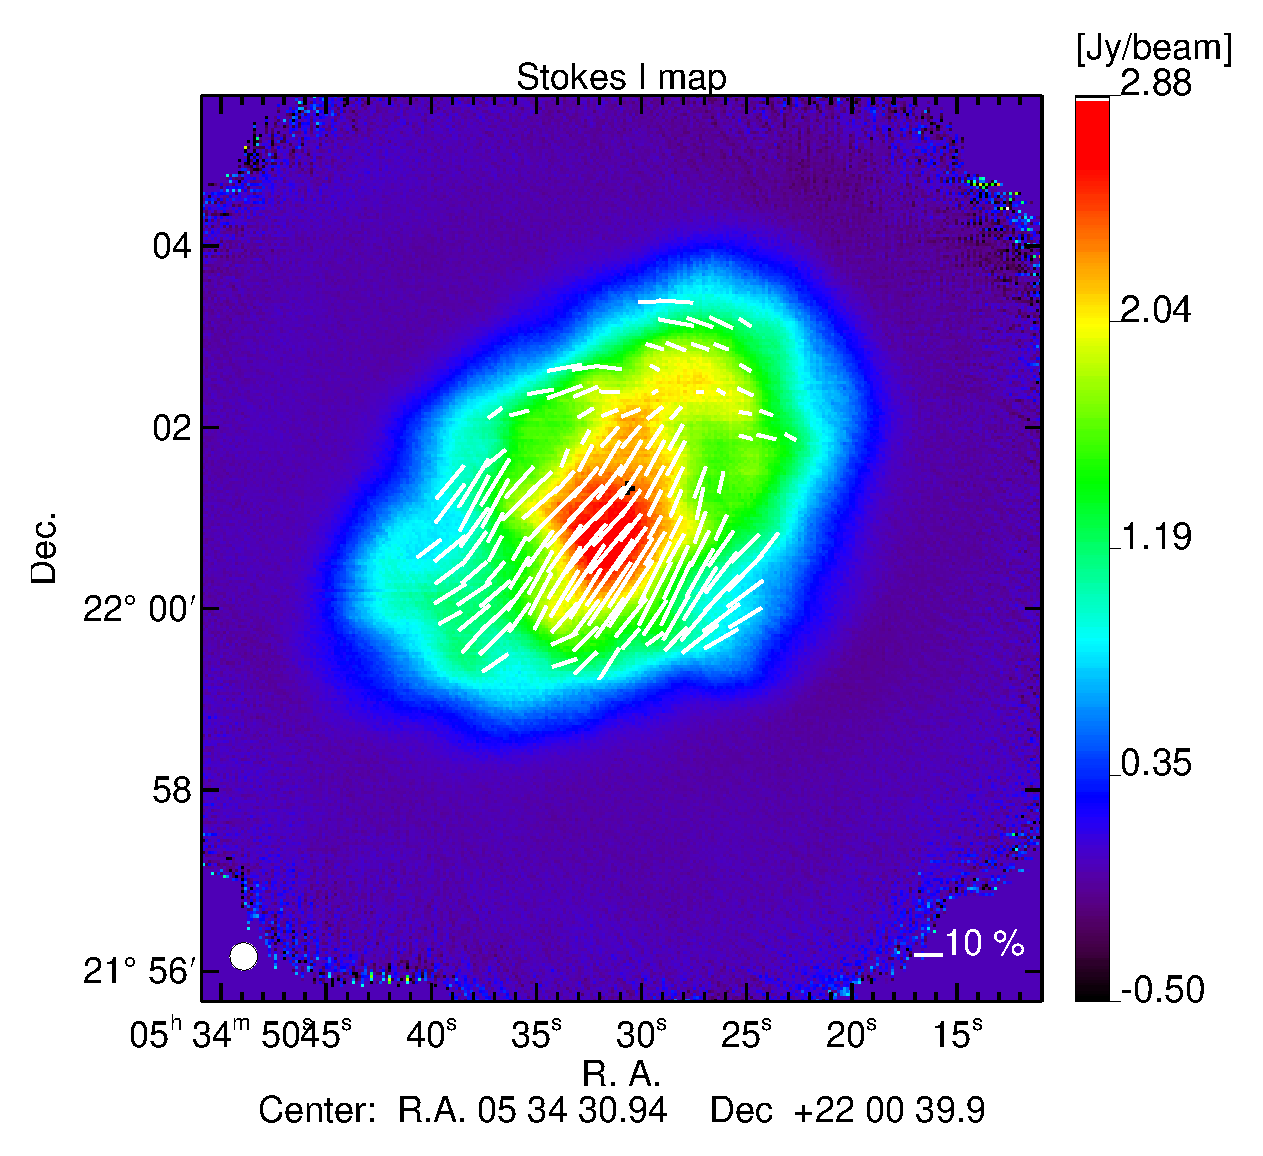
\includegraphics[width=0.32\linewidth,keepaspectratio]{figures/Crab_I_map2_2mm.pdf}}	
	     { 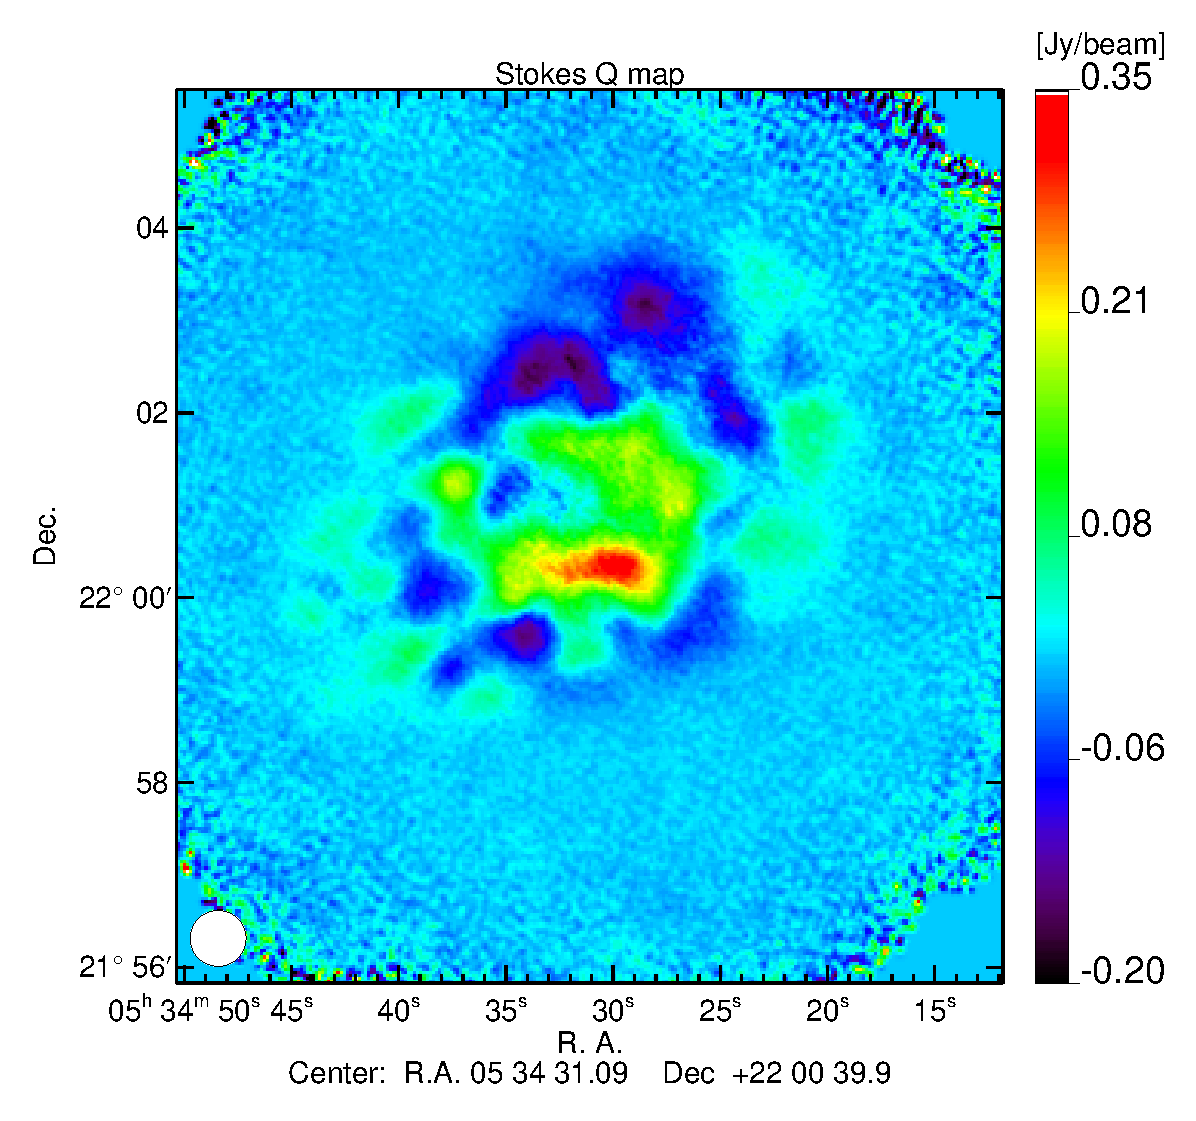
\includegraphics[width=0.32\linewidth,keepaspectratio]{figures/Crab_Q_map2_2mm.pdf}}
          { 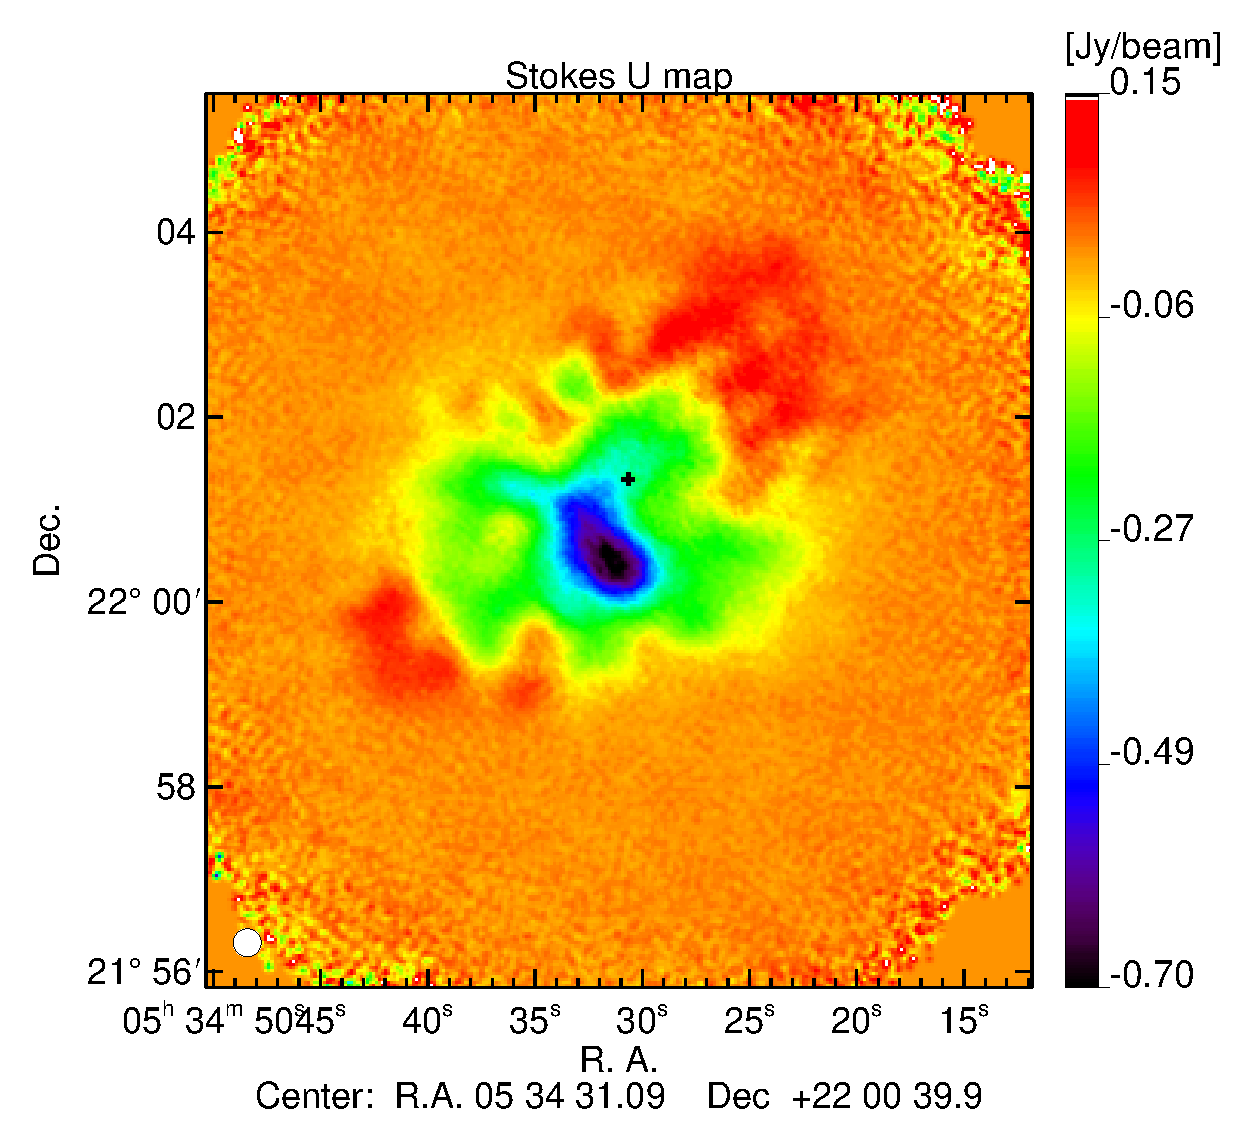
\includegraphics[width=0.32\linewidth,keepaspectratio]{figures/Crab_U_map2_2mm.pdf}} 
           \caption{From left to right: Crab nebula Stokes $I$, $Q$ and, $U$ maps obtained at 150 GHz with the \NIKA\ camera. Polarization vectors, indicating both the degree and the orientation, are over-plotted in black on the intensity map where the polarization intensity satisfies P $\textgreater$  3 $\sigma_P$, where $\sigma_P$ represents the uncertainty in P. }
\label{crab_intensity_maps}
\end{figure*}


\section{Introduction}\label{sec:introduction}
The polarization of the Cosmic Microwave Background (CMB) anisotropies offers a powerful way to investigate the early Universe. They can be decomposed into a scalar and a pseudo-scalar field, respectively called $E$  and $B$ modes. The primordial density fluctuations (scalar perturbations) can only produce $E$ CMB polarization, while $B$ CMB polarization can only be produced by 
primordial (tensor perturbations) gravitational waves \citep{polnarev1985polarization, 1997PhRvL..78.2054S} arising from the inflationary epoch \citep{PhysRevD.23.347, linde1982new} and by gravitational lensing of the $E-$modes \citep{ade2015planck}.
The detection of the primordial $B-$modes could definitively probe the existence of an inflationary epoch and constitutes one of the most ambitious goals of the modern observational cosmology.

Recently, \citet{bicepplanck2015,bicep2016} set a 95\% upper limit for the detection of the tensor to scalar ratio $r$ $\textless$ 0.07.
Upcoming CMB experiments aiming at measuring the primordial $B-$modes require an accurate determination of the foreground emissions to the CMB signal and a high control of the systematic effects. One of the most difficult parameters to be characterized for a CMB polarization experiment is the calibration of residual cross polarization and of the absolute polarization angle. This can be achieved using observations of well known polarized sources like the Crab nebula.

The Crab Nebula (or Tau A) located at equatorial coordinates $R.A. = 5^h34^m32s$ and $Dec. = 22^{\circ}0^{\prime}52^{\prime\prime}$ is a plerion-type supernova remnant emitting a highly polarized signal.
A synchrotron emission from the nebula is observed in the radio frequency domain, which is powered by a pulsar through its jet. 
Moreover, near the center of the nebula we observe a shock, which is formed where the jet is thermalized and ultra-relativistic particles are released into the surrounding nebula \citep{2000ApJ...536L..81W,2011A&A...528A..11W}. 

This source represents the most intense polarized astrophysical object in the microwave sky at angular scales of few arcminutes and for this reason it is of particular interest  for the calibration of CMB polarization experiments, which have widths beam comparable to the extension of the source.
For a more detailed review on this source we refer to \citet{2008ARA&A..46..127H}.

The Crab nebula is used for polarization cross-check analysis in the frequency range from 30 to 353 GHz. High angular resolution observations from the XPOL experiment \citep{thum2008} at the IRAM 30 m telescope have revealed the spatial distribution of the Crab Nebula in intensity and polarization at 90 GHz with an absolute accuracy of 0.5$^{\circ}$ in the polarization angle \citep{aumont2010}. 
High angular resolution observations of the Crab nebula in polarization could be very useful for the calibration of the next generation of polarization experiments. In particular those aiming at a precise measurement of the CMB polarization, which have a large frequency range to be able to carefully study foreground emission \citep{2016IJMPD..2540008K}. 

Previous studies \citep{macias2010} of the total flux density of the Crab nebula have shown a spectrum well described by a single synchrotron component, and predict negligible variations in polarization fraction and angle in the frequency range of interest for CMB studies.
 
Polarized observations of the Crab Nebula have been performed with the \NIKA\ camera \citep{monfardini2010,catalano2014,monfardini2014} at the IRAM 30 m telescope during the observational campaign of February, 2015. A first overview in \NIKA\ Crab polarization observations was given in \cite{2016JLTP..184..724R}. In this paper we go a step forward in the analysis and combine the \NIKA\ observations with previous ones.
In order to trace the polarized Spectral Energy Density (SED) we use polarization observations from the WMAP satellite at 23, 33, 41, 61 and 94 GHz \citep{2011ApJS..192...19W}, from the \Planck\ satellite at 30, 44, 70, 100, 143, 217, 353 GHz and from XPOL at 90 GHz \citep{aumont2010}. 
 The paper is organized as follows: in Sec.~\ref{sec:NIKA observations} the intensity and polarization maps obtained with the \NIKA\ camera are presented together with the polarization degree and angle spatial distribution; Sec.~\ref{sec:Polarization estimates in CMB experiments like beams} presents the reconstruction of the polarization properties in well defined regions; Sec.~\ref{sec:Polarization intensity Spectral Energy Density (SED)} presents the Crab nebula SED; in Sec.~\ref{sec:conclusions} we draw conclusions.
 \begin{figure*}
\centering
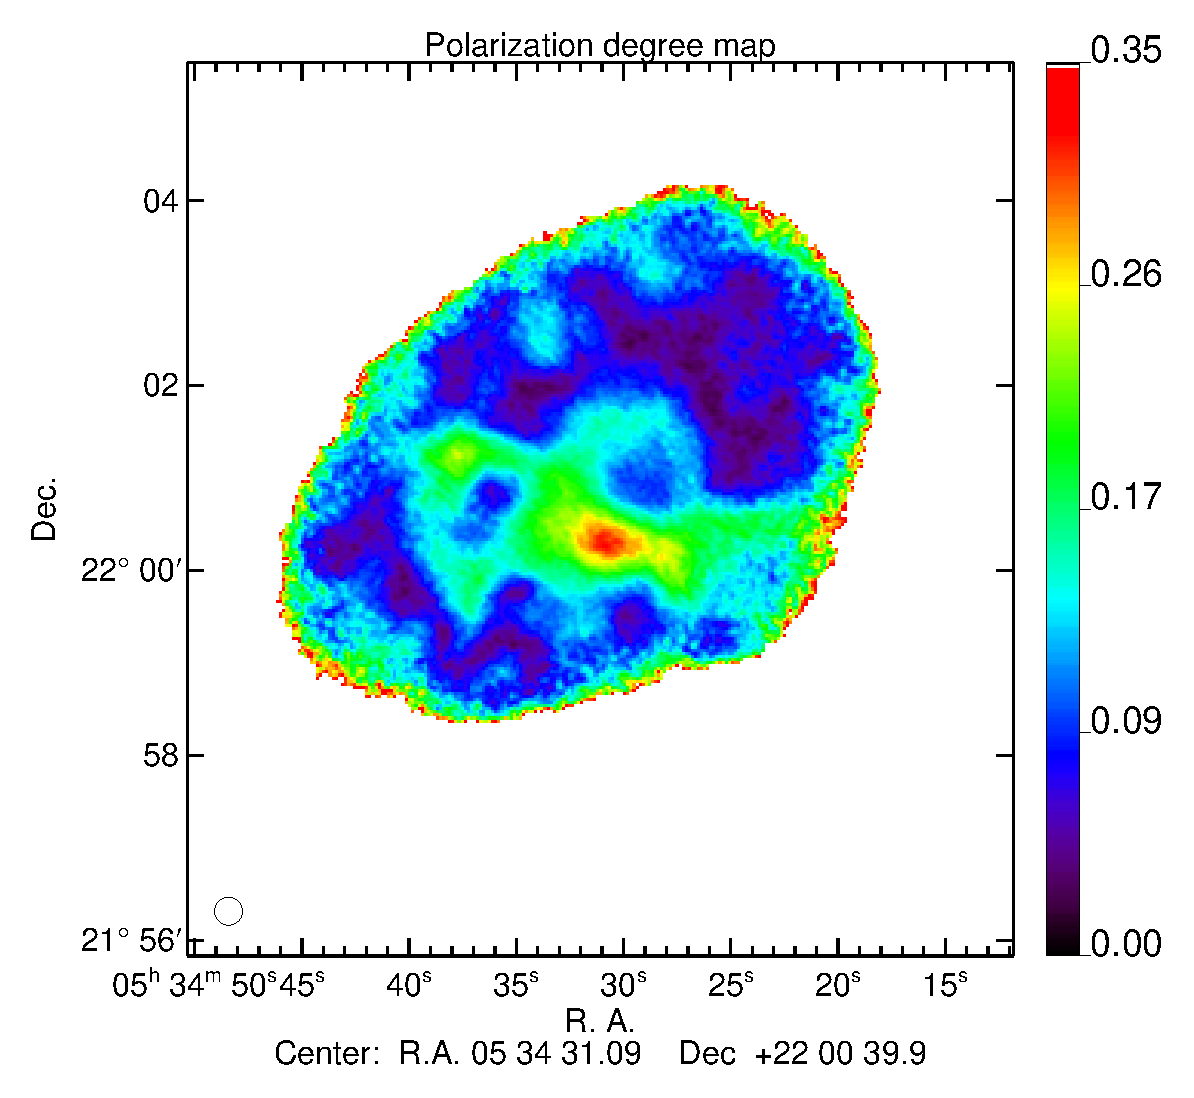
\includegraphics[clip, angle=0, scale = 0.35]{figures/Crab_pol_deg2_2mm.pdf}
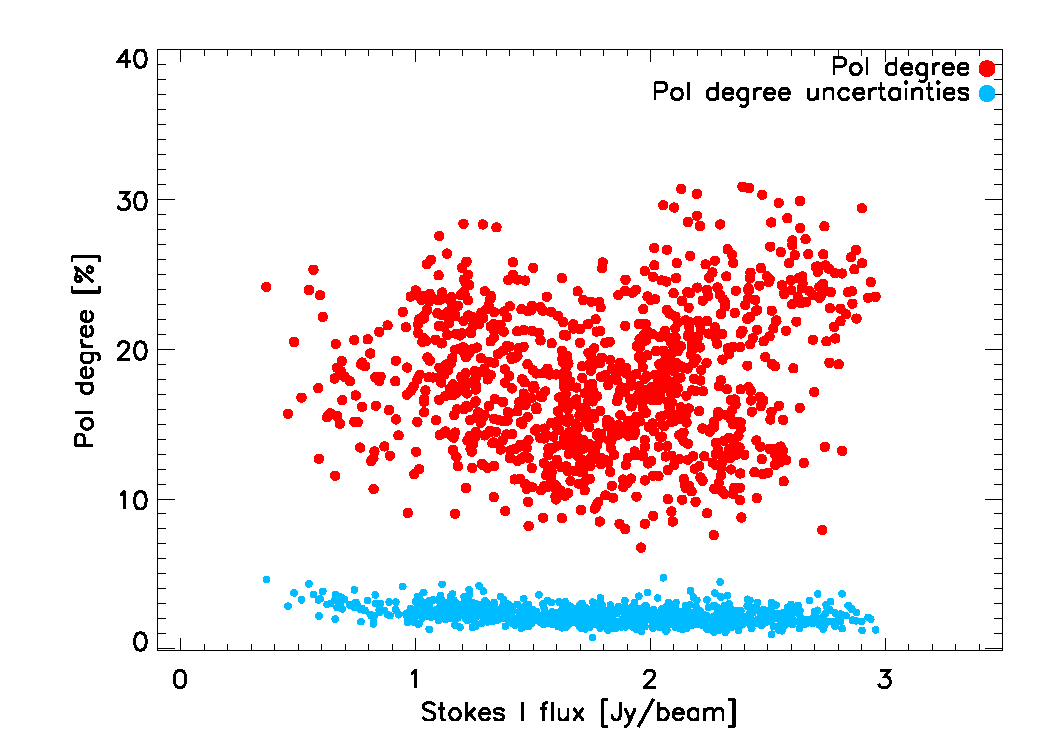
\includegraphics[clip, angle=0, scale = 0.5]{figures/pol_deg_vs_I_2mm.pdf}
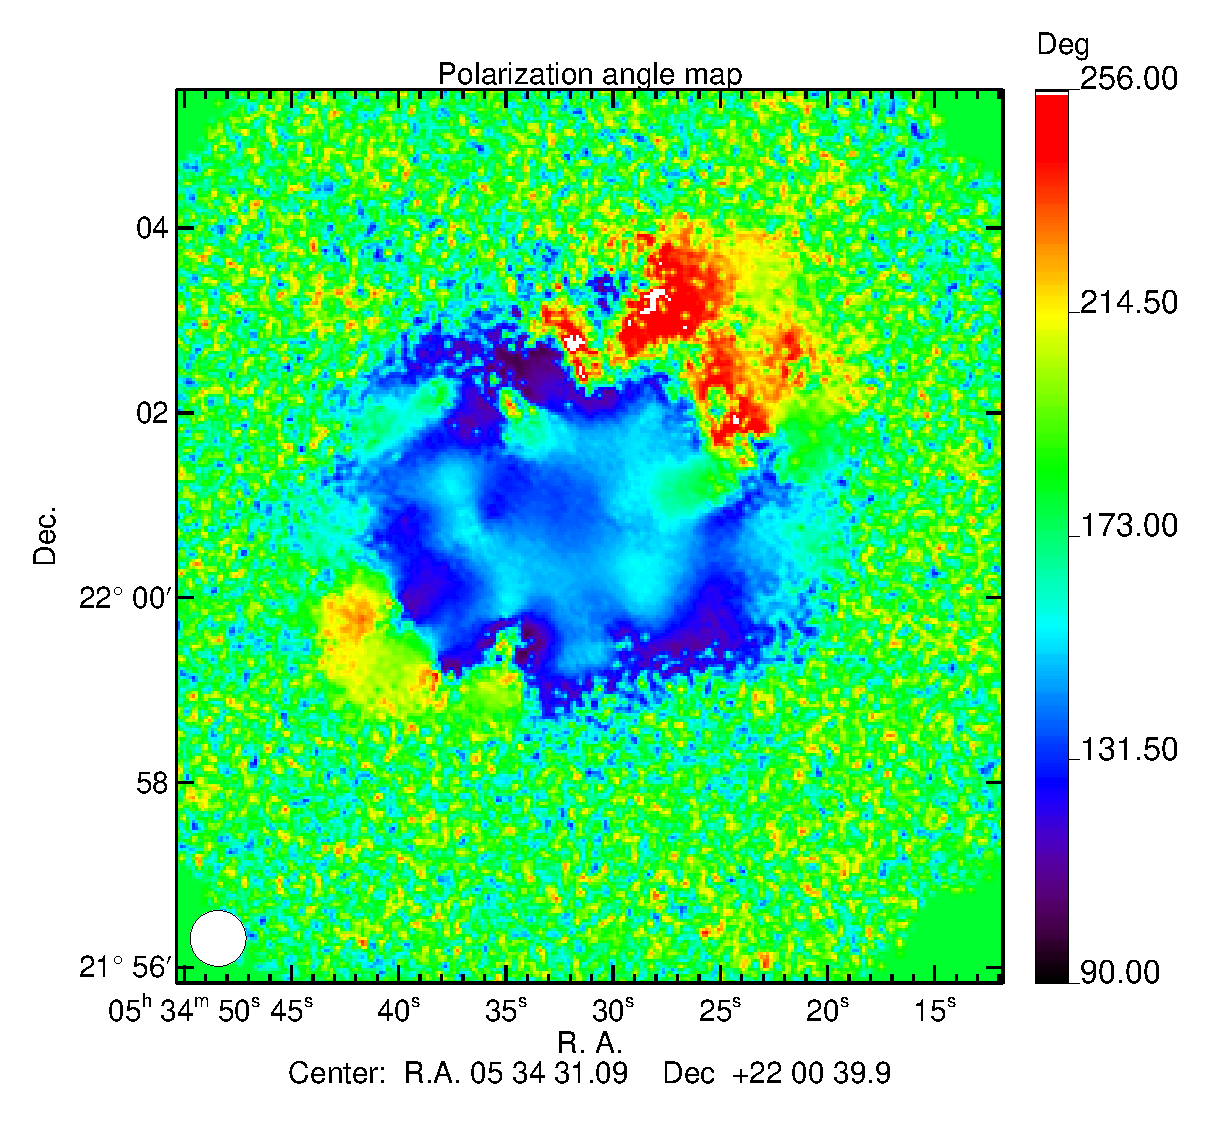
\includegraphics[clip, angle=0, scale = 0.35]{figures/Crab_angle2_2mm.pdf}
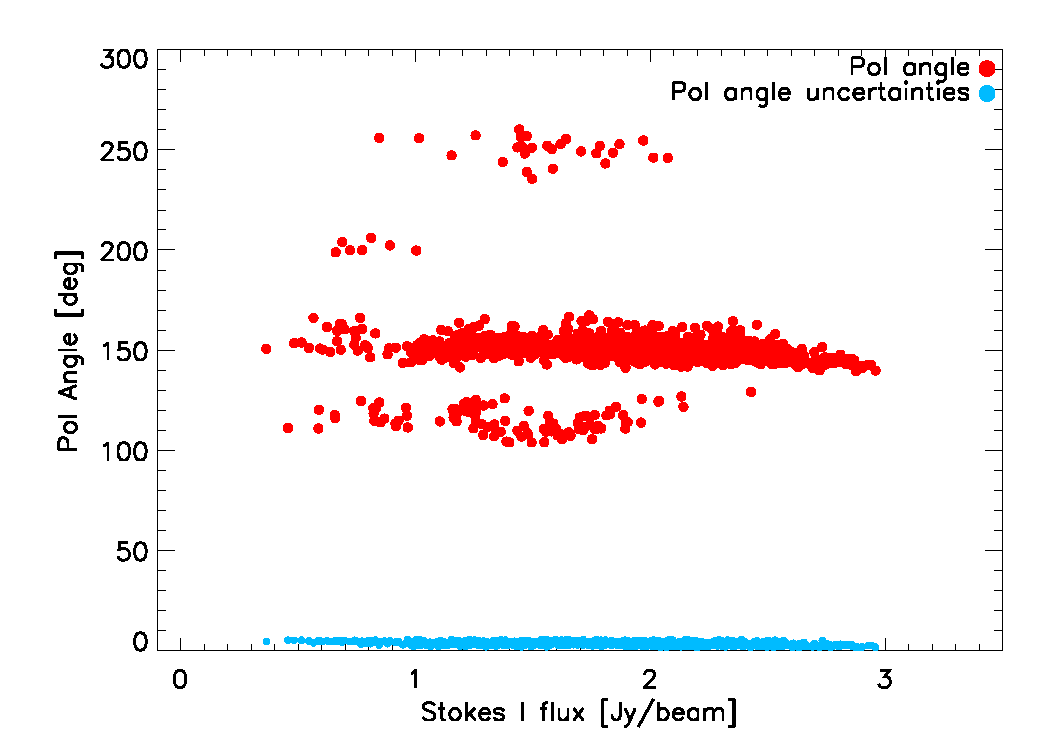
\includegraphics[clip, angle=0, scale = 0.5]{figures/pol_angle_vs_I_2mm.pdf}
\caption{{\it Top}: polarization degree naive estimator map $p$ (left) of the Crab nebula. Noise bias corrected values of $p$ are represented on the right panel as a function of the Stokes $I$ total intensity map where the polarization intensity $P$ $\textgreater$ 5$\sigma_{P}$. {\it Bottom}: polarization angle map $\psi$ (left) of the Crab nebula. Polarization angle $\psi$ where $P$ $\textgreater$ 5$\sigma_{P}$ vs the Stokes $I$ total intensity map. The cyan dots represent the uncertainties calculated as the dispersion between different scans.}
\label{fig:pol_degree}
\end{figure*}
 \begin{figure}
  \centering
     	   {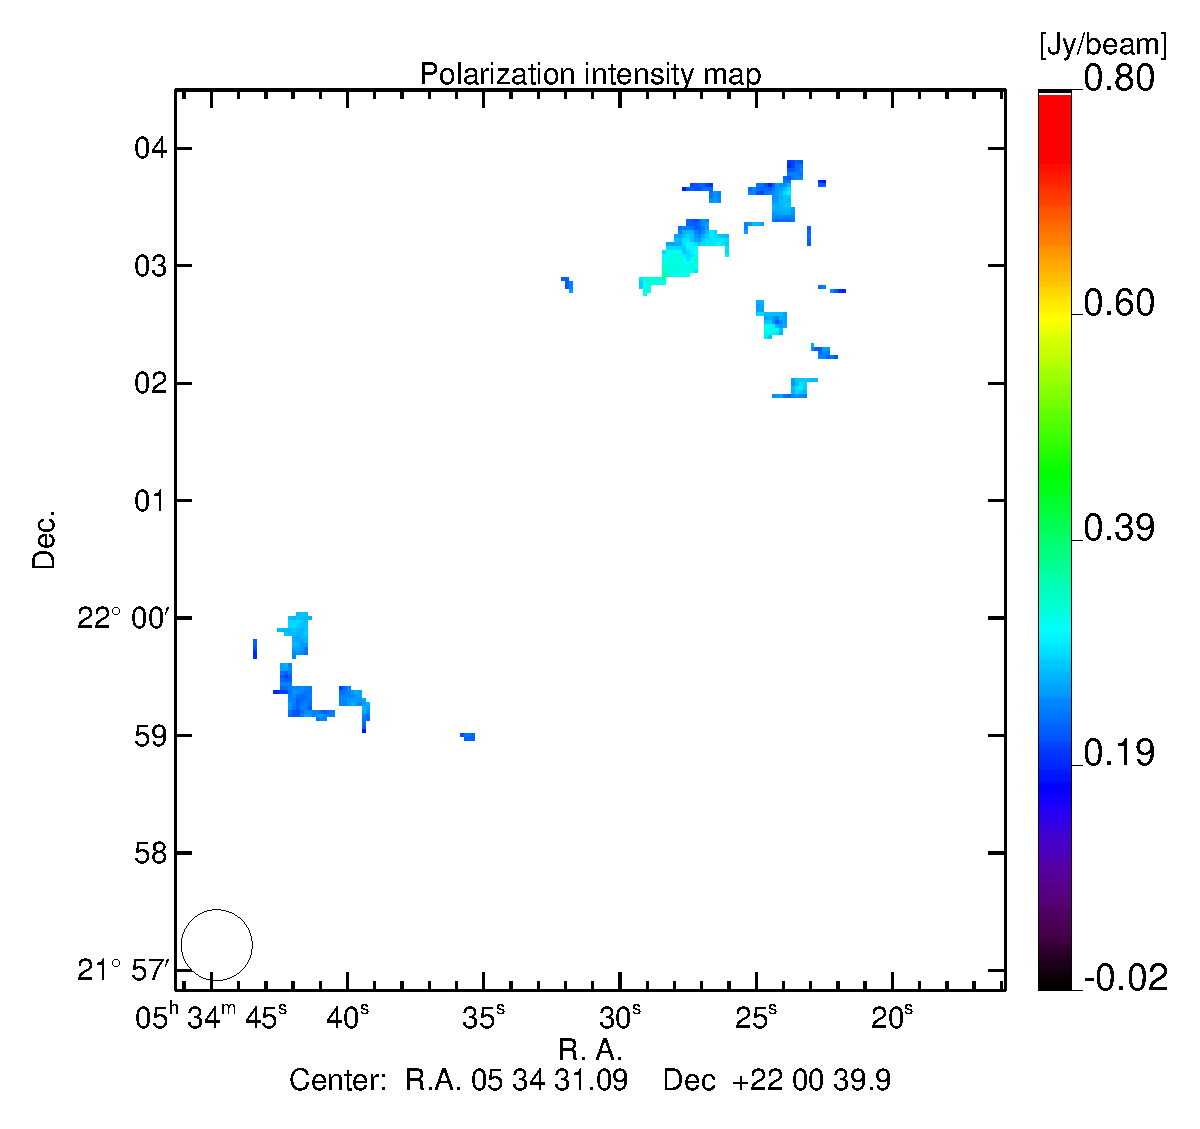
\includegraphics[width=0.75\linewidth,keepaspectratio]{figures/Crab_ipol2_2mm.pdf}}
\caption{Polarization intensity map obtained at 150 GHz. The map shows high polarized emission reaching a value of 0.8 Jy beam$^{-1}$.}
\label{crab_ipol_maps}		
  \end{figure}
 

\section{\NIKA\ observations of the Crab Nebula}\label{sec:NIKA observations}
\subsection{\NIKA\ camera}\label{sec:nika camera}
\NIKA\ is a dual band camera observing the sky at 150 and 260 GHz with 18$^{\prime\prime}$ and 12$^{\prime\prime}$ FWHM resolution, respectively. It has been operated at the IRAM 30 m telescope between 2012 and 2015. A detailed description of the \NIKA\ camera can be found in \citet{monfardini2010, monfardini2011} and \citet{catalano2014}. In addition to intensity observations it was also a test bench for polarization facilities of the final instrument \NIKAd, installed at the telescope in October, 2015 \citep{calvo2016,2016arXiv160508628C}.
 In \cite{ritacco2017} we give more details on the \NIKA\ polarization facilities and it describes the performance of the instrument at the telescope. The characterization of the \NIKA\ polarization capabilities has been very important to get prepared for the follow-up camera \NIKAd. Beyond that, \NIKA\ provided the first polarization observations performed with Kinetic Inductance Detectors, which represent a suitable detector technology for the development of the next generation of CMB experiments.
%Unfortunately, the observations of the Crab nebula performed at 260 GHz have been limited by the sensitivity of the \NIKA\ instrument in polarization and the resulting maps show a no significant detection, for that reason here we discuss only the observations performed at 150 GHz. 

\subsection{\NIKA\ observations}\label{sec:nika_observations}
Polarization measurements with the \NIKA\ camera have been carried out with a combined action of a continuously rotating metal-mesh Half Wave Plate (HWP), a polarizer and KIDs arrays mounted inside the \NIKA\ instrument. 
Since \NIKA\ detectors \citep{roesch2012} are not sensitive to the linear polarization a polarizer is necessary to select one direction of it. 
Crab nebula polarization observations with the \NIKA\ camera have been performed at the IRAM 30 m telescope during the observational campaign of February, 2015. Fig.~\ref{crab_intensity_maps} shows the Stokes $I$, $Q$ and $U$ maps obtained by a co-addition of 16 on-the-fly maps of 8 $\times$ 6 arcminutes for a total observation time of $\sim$ 2.7 hours. The maps were performed in equatorial coordinates according to four different scan directions: 0$^{\circ}$, 90$^{\circ}$, 120$^{\circ}$, 150$^{\circ}$. This allowed us to have the best covering of the source. 
The polarization maps represented in Fig.~\ref{crab_intensity_maps} have been obtained through a dedicated data reduction pipeline. The already existing \NIKA\ pipeline \citep{catalano2014,adam2013} developed for intensity observations has been extended to polarization measurements. The first step of this dedicated module sees the subtraction of the a parasite signal which is modulated at harmonics of the HWP rotation frequency and represents the most annoying noise contributing to the polarized signal. 
The second step is the reconstruction of the Stokes $I$, $Q$ and $U$ time ordered information (TOI) from modulated data. This is achieved using a demodulation procedure consisting in a lock-in around the fourth harmonic of the HWP rotation frequency, where the polarization signal is located. Finally, an intensity to polarization leakage effect was observed on the observation of an unpolarized source, the planet Uranus, and corrected by developing an algorithm able to reduce the effect from $\sim$ 3\% to lower than 1\%. More details on this effect and the data analysis pipeline can be found in \cite{ritacco2017}.
For the Crab nebula observations the leakage systematic effect reaches a value of 0.5\% peak-to-peak of the total intensity.
The level of this spurious instrumental polarization appears significantly lower on an extended source than on Uranus. 
This can be due to a compensation of the negative and positive signal between adjacent pixels. Although the effect is weaker the algorithm of correction is still applied to obtain the final maps represented in Fig.~\ref{crab_intensity_maps}.

In order to have a proper estimate of the polarization degree we need to have a proper reconstruction of the intensity map. For an extended source like the Crab nebula, with angular size larger than the \NIKA\ FoV, it is difficult to correctly estimate its intensity emission avoiding filtering effects due to noise decorrelation methods. A common mode decorrelation method consisting on a template reconstruction (to be subtracted) using only the pixels outside the source is usually used in \NIKA\ data analysis. Filtering effects can be encountered in regions where the number of pixels used for the template reconstruction is too low.
In order to avoid such an effect the Stokes $I$ map shown on the left panel of Fig.~\ref{crab_intensity_maps} has been obtained by using a decorrelation method called ``dual-band decorrelation''. Such a decorrelation algorithm has been developed for the reconstruction of the Sunyaev-Zel'dovich signal in galaxy clusters observations \citep{adam2013} taking advantage of \NIKA\ dual-band capabilities. The idea of this algorithm arises with the fact that the atmospheric emission is stronger at 260 GHz than at 150 GHz, as a consequence we can use 260 GHz observations as a ``template'' of the atmospheric emission to be subtracted to the 150 GHz observational data.
 


 %The level of this spurious instrumental polarization is significantly lower than the observed one on Uranus. This is probably due to a compensation of the negative and positive signal between adjacent pixels. Although the leakage effect is very weak on this diffuse source the correction is still applied to produce the final maps presented in Fig.~\ref{crab_intensity_maps}.


%This data analysis allows to produce Stokes $I$, $Q$ and $U$ maps as shown in Figg.~\ref{crab_intensity_maps},\ref{crab_polarization_maps}. The continuos rotation of the HWP running at 2.98 Hz permits to shift the polarized signal at higher frequencies. In this way the polarized signal is cleaned by the low frequency noise (e.g.~atmosphere variations, electronics etc), but the intensity signal could be. As a consequence an accurate determination of the polarization fraction requires a good estimation of the total intensity map. 

%Fig.~\ref{crab_intensity_maps} shows the Stokes intensity map obtained at 150 GHz using the dual band decorrelation method.


%For illustration we show in Fig.~\ref{fig:crab_leakage_maps} the intensity to polarization leakage maps of Stokes $Q$ and $U$ of the Crab nebula, obtained as subtraction of the $Q$ and $U$ maps before and after leakage correction.

%\begin{figure}[h!]
%\begin{center}
%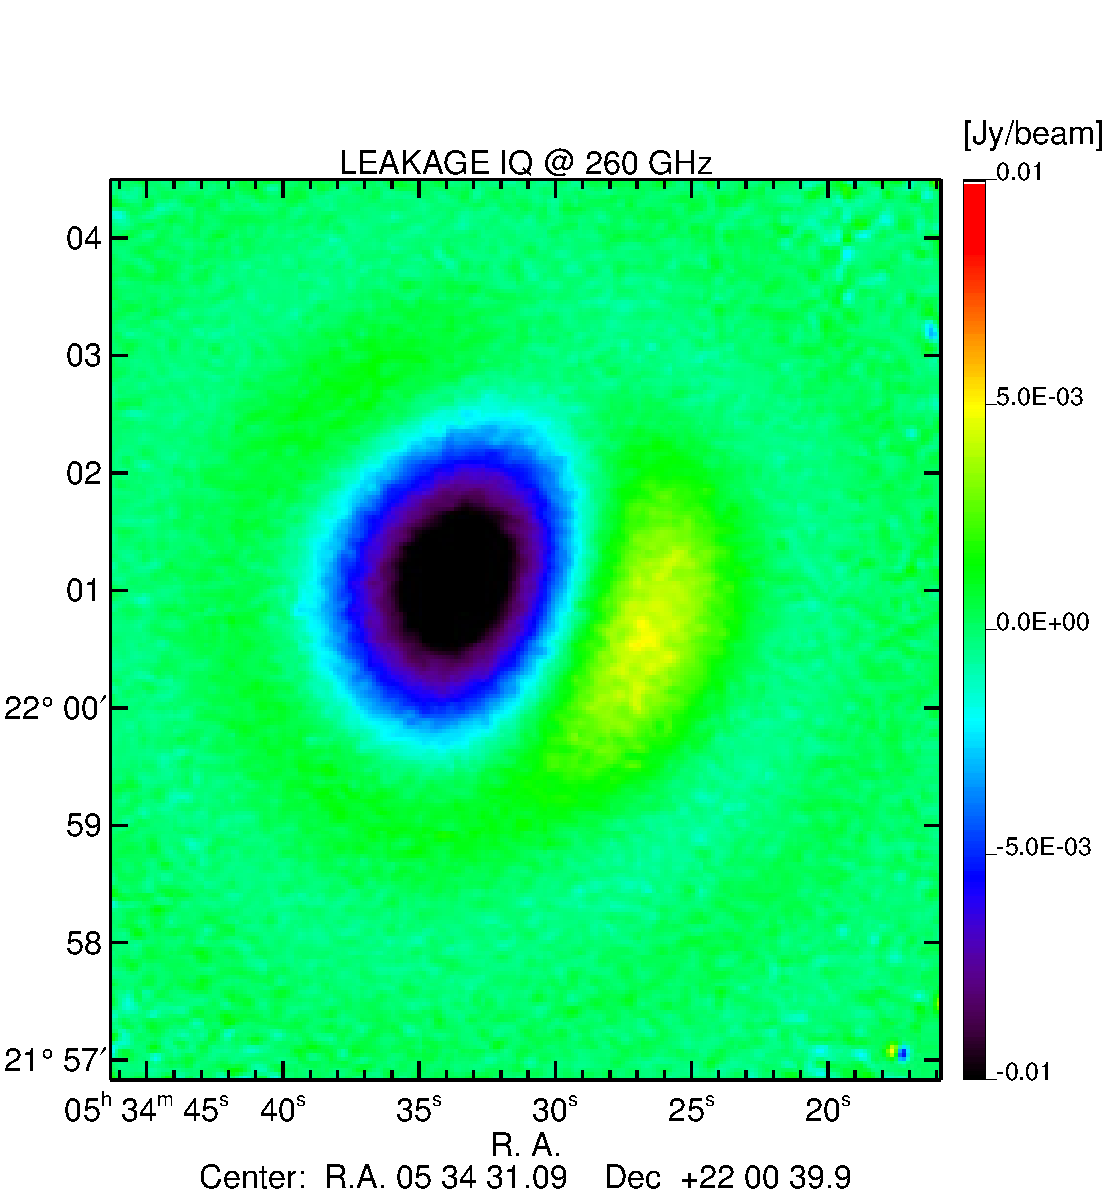
\includegraphics[clip, angle=0, scale = 0.23]{figures/Crab_IQ_1mm.pdf}
%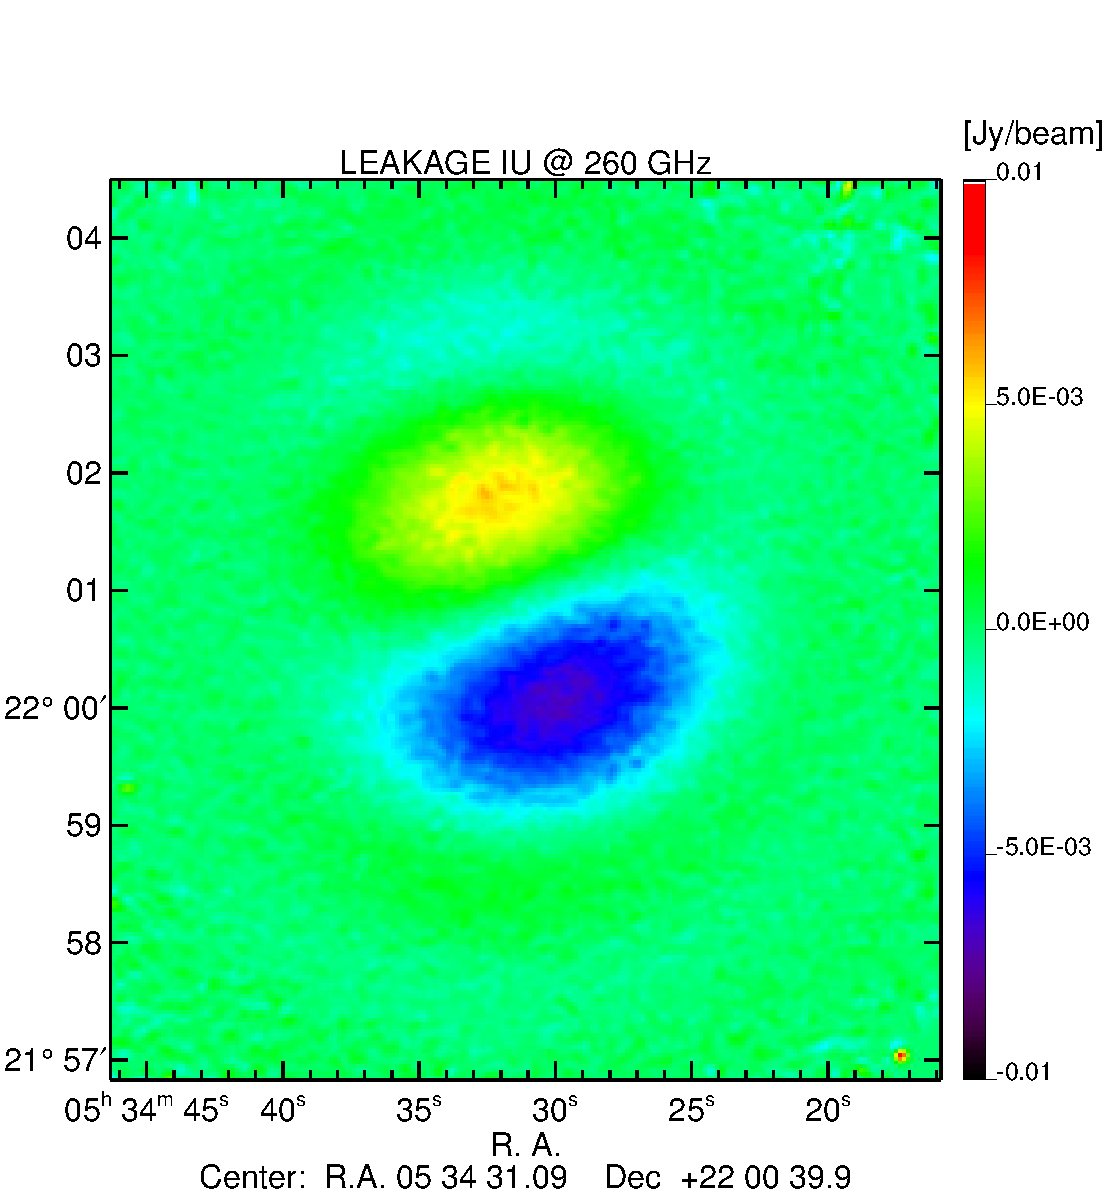
\includegraphics[clip, angle=0, scale = 0.23]{figures/Crab_IU_1mm.pdf}

%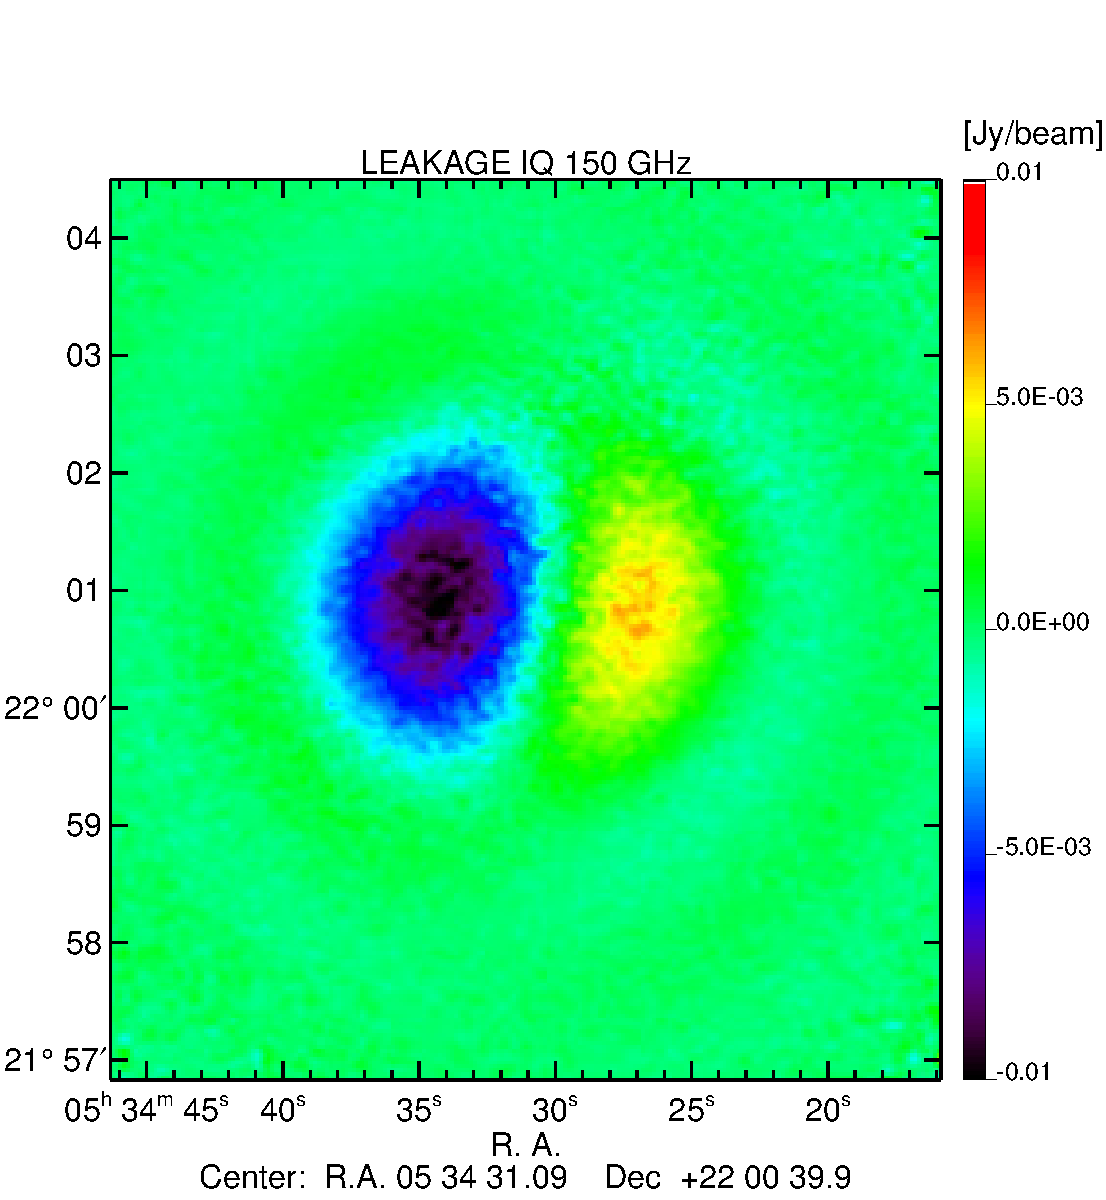
\includegraphics[clip, angle=0, scale = 0.23]{figures/Crab_IQ_2mm.pdf}
%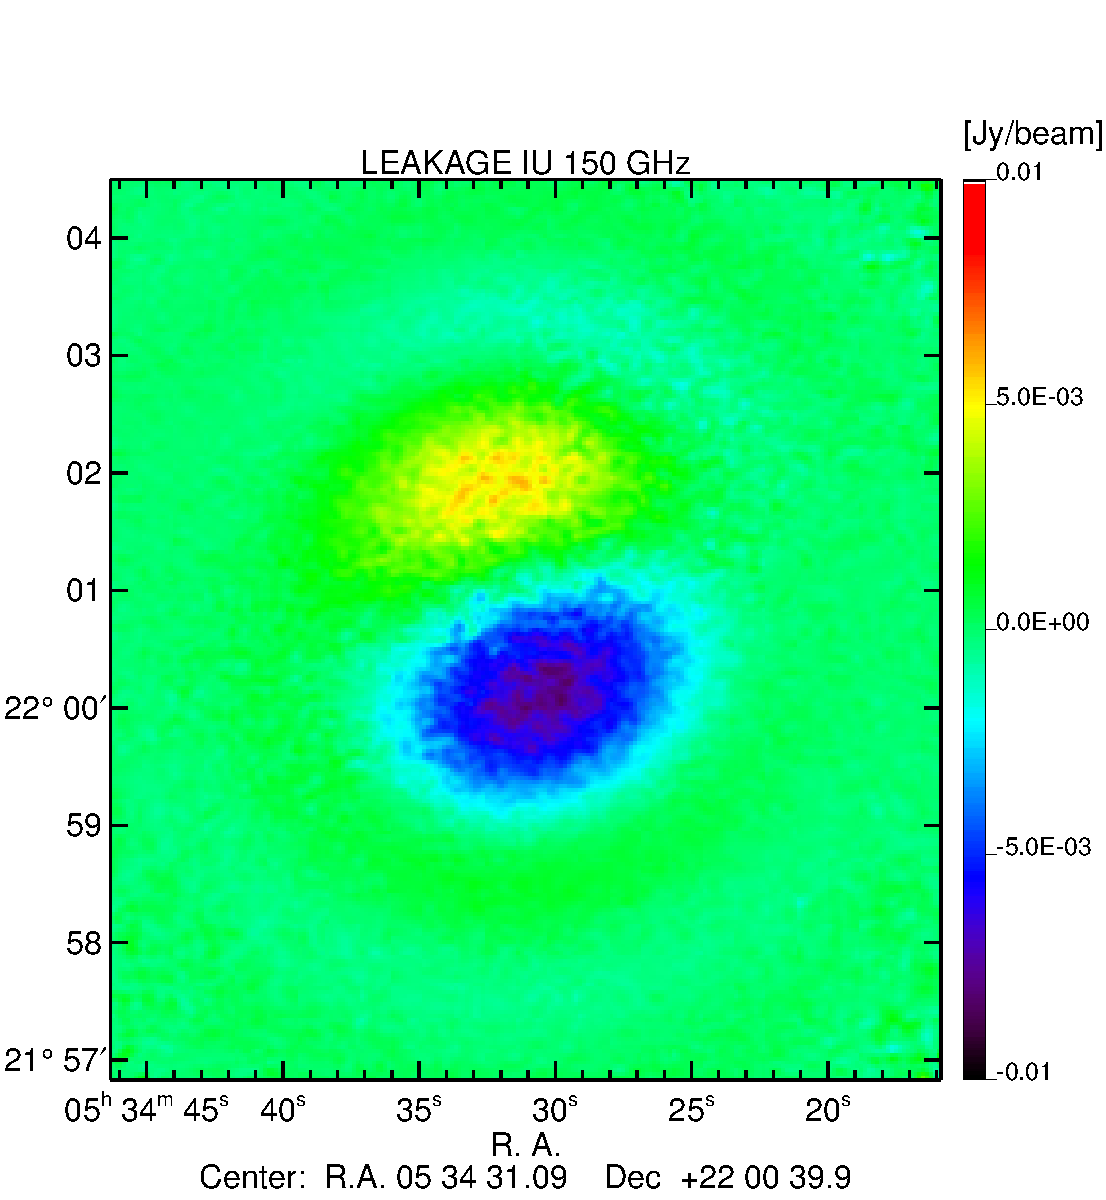
\includegraphics[clip, angle=0, scale = 0.23]{figures/Crab_IU_2mm.pdf}
%\caption{Crab Nebula Stokes $Q$ and $U$ intensity to polarization leakage maps. The peak-to-peak estimation reaches a value 0.5\% of the total intensity emission, respectively. See the total intensity map represented in Fig.~\ref{crab_intensity_maps}.}
%\label{fig:crab_leakage_maps}
%\end{center}
%\end{figure}

%The intensity to polarization leakage peak-to-peak reaches a value of $\sim$ 1\% (260 GHz) and 0.5\% (150 GHz) of the total intensity, see Fig.~\ref{fig:crab_leakage_maps}. 

\subsection{Crab polarization properties}\label{sec:pol_properties}
In this section we discuss the polarization properties of the source in terms of polarization degree $p$ and angle $\psi$, which are defined through the Stokes parameters $I, Q$, and $U$ as follows:
\begin{eqnarray}
 p    &=& \frac{\sqrt{Q^2 + U^2}}{I} \nonumber \\
 \psi &=& \frac{1}{2}\arctan\frac{U}{Q}.\label{angledegree_polar}
 \end{eqnarray}
 These definitions are not linear in $I$, $Q$ and $U$ and are biased by the noise. Where the signal-to-noise ratio is too low ($\it{i.e.}$ $ Q \simeq U \simeq 0$)  the noise measured on $Q$ and $U$ maps will yield a non-zero degree of the polarization estimate.
\citet{1980A&A....91...97S,1985A&A...142..100S,montier} proposed analytical solutions to correct this bias. At the limit of high S/N ratio which the estimation of the polarization degree and its uncertainty become:
 \begin{eqnarray}
 p    &=& \frac{\sqrt{Q^2 + U^2 - \sigma_{Q}^2 - \sigma_{U}^2}}{I}, \nonumber \\ 
  \sigma_{p} &=& \frac{\sqrt{Q^2\sigma_Q^2 + U^2\sigma_U^2 + p^4I^2\sigma_I^2}}{pI^2}.
  \label{p_true_degree}
 \end{eqnarray}
 Furthermore, the polarization angle in a high S/N regime can be approximated by the classical Eq.~\ref{angledegree_polar} with uncertainty
  \begin{eqnarray}\label{angle_uncertainty}
  \sigma_{\psi} = \frac{\sqrt{Q^2\sigma_Q^2 + U^2\sigma_u^2}}{2(pI)^2}.
  \end{eqnarray}

The polarization degree $p$ spatial distribution of the Crab nebula, without correction for noise bias, is represented on the top left panel of Fig.~\ref{fig:pol_degree}. The polarization reaches 35 \% of the intensity across the peak of the intensity signal  and decreases going towards the edges of the source. 
This feature highlights the interest of high resolution polarization observations of the Crab nebula. Moreover, the right panel of the figure shows the polarization degree $p$ as function of the Stokes total intensity $I$ map. Here the values have been bias corrected and satisfy the condition P=$\sqrt{Q^2+U^2}$ $\textgreater$ 5 $\sigma_P$. The distribution of the polarization degree in Fig.~\ref{fig:pol_degree} appears highly dispersed around a polarization degree value of $\sim$ 20-30$\pm$4\%.

The bottom left panel of Fig.~\ref{fig:pol_degree} shows  the polarization angle $\psi$ spatial distribution, which has not been corrected for noise bias. 
We observe a relatively constant polarization angle, about 150 $^{\circ}$ represented here in equatorial coordinates, except for the northern region where the averaged angle is around $220^{\circ}$. 
These values are confirmed by the bottom right panel, which show the polarization angle distribution as a function of the total intensity. Here the value have been bias corrected and satisfy the condition P=$\sqrt{Q^2+U^2}$  $\textgreater$ 5 $\sigma_P$.

The sudden change of the polarization angle on the northern region was already observed by the XPOL experiment at 90 GHz \citep{aumont2010}.
This together with the variation of the polarization fraction discussed above confirms the need of high angular resolution observations at low and high frequencies for a good understanding of the Crab polarized emission.

The polarization intensity $P$ map, represented in Fig.~\ref{crab_ipol_maps}, exhibits a polarized emission peaked at 0.8 Jy beam$^{-1}$ and decreasing to 0.1 Jy beam$^{-1}$ on the extremities of the nebula. 

\section{Total intensity and polarization fluxes}\label{sec:Polarization estimates in CMB experiments like beams}
We compute in this section the total intensity flux across the Crab nebula, which has an extension of about  4$^{\prime}$ as shown in Fig.~\ref{crab_intensity_maps}.
We use standard aperture photometry techniques to calculate the flux up to 4$^{\prime}$ as shown in Fig.~\ref{crab_integrated_flux}. We use as center position the center of the map. A zero level in the map, calculated as the mean of the signal measured on an external annular ring region, has been subtracted from the flux. The total signal estimated is 204.4$\pm$7.9$\pm$10.2 Jy. The uncertainty accounts for statistical uncertainty computed from fluctuations of the signal at large radii. The second term of the uncertainty indicates the calibration error corresponding to  $\simeq$ 5\% at 150 GHz. This absolute calibration error is estimated from the dispersion of the estimated flux of Uranus for observations collected during the same observational campaign.

\begin{figure}[h!]
  \centering
     { 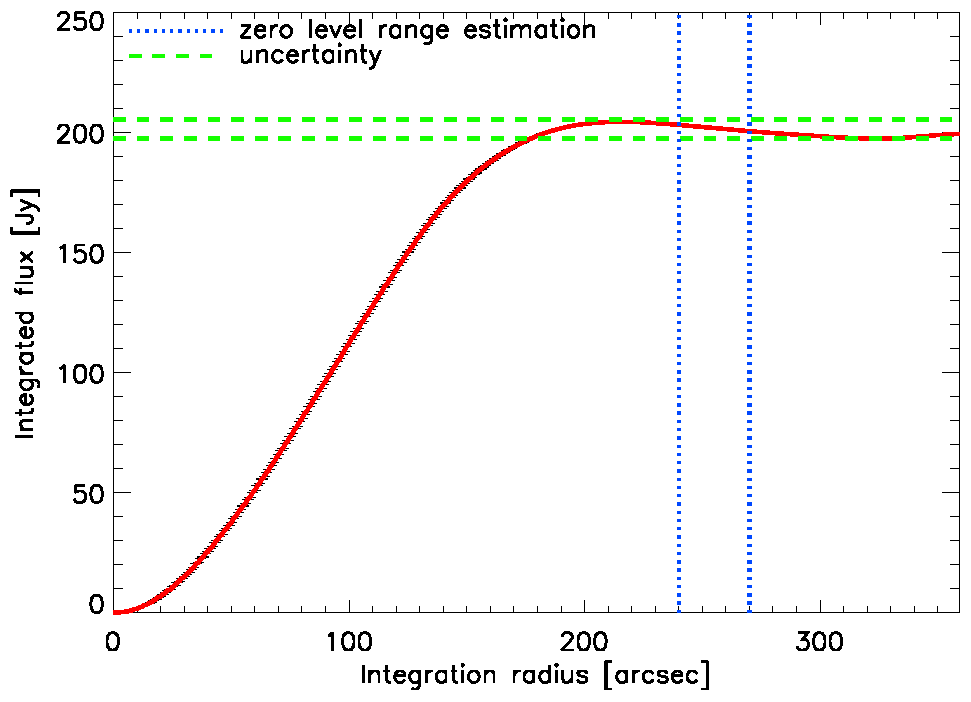
\includegraphics[width=0.85\linewidth,keepaspectratio]{figures/Crab_integrated_flux_2mm.pdf}}
     \caption{Cumulative flux of the Crab nebula at 150 GHz. The flux has been corrected by a zero level in the map, which corresponds to the mean of the signal calculated in an annular ring indicated by the blue dotted lines. The green dotted line represents the uncertainties measured at large radii.}
\label{crab_integrated_flux}
\end{figure}


In order to compare with low angular resolution CMB experiments we also give the polarization degree $p$ and angle $\psi$ integrated values obtained in well defined regions. 
Tab.~\ref{tab:crab_results} shows the total intensity $I$, polarized intensity $P$, polarization degree $p$ and polarization angle $\psi$ obtained in four different regions. In order to compare with the \Planck\ satellite we estimate the values in two regions of $7^{\prime}$ and $5^{\prime}$ corresponding to the beams of the \Planck\ frequency channels at 143 and 217 GHz, respectively. 
Further, two other regions are defined with high S/N ratio. First, where $P$ $\textgreater$ $3\sigma_P$ and  where $P$ $\textgreater$ 0.2 Jy. 
In Tab.~\ref{tab:crab_results} the polarization angles are represented in Galactic coordinates to ease the comparison with the \Planck\ \citep{2015arXiv150702058P} and \WMAP\ CMB experiments \citep{2011ApJS..192...19W}. 

Fig.~\ref{crab_p_angle_comparison} shows the polarization fraction (top) and angle (bottom) as function of the frequency for five different instruments: \Planck, WMAP, XPOL, SCUPOL and \NIKA.
For \NIKA\ we have averaged within a 5$^\prime$ region and considered only pixels for which $P$ $\textgreater$ $3\sigma_P$. Notice that SCUPOL maps \citep{scubapol} provided at 352 GHz have reduced angular size w.r.t \NIKA. In order to compare with it we define a small region of 1.4$^\prime$ around the peak of the polarization intensity. 
For the polarization fraction we keep the convention used by XPOL \citep{aumont2010} and we represent in the figure the value measured in 5$^{\prime}$. 
The solid line in both figures represents the mean value found using all the observations shown and the uncertainty represents the standard deviation. 

\begin{table*}
  \centering
      \begin{tabular}{ccccccccc}
      \hline
      \hline
       & $I$ & $P$ & $p$ & $\psi$  \\ 
                                         & [Jy]         &    [Jy]         & [\%]  & [$^\circ$] \\
      \hline
      \hline
 seen by 7$^{\prime}$   & 231.8$\pm$0.2  & 14.03$\pm$0.09 & 6.05$\pm$0.04 & -85.1$\pm$0.5$\pm$1.8(syst)  \\ 
    
            seen by 5$^{\prime}$ & 219.0$\pm$0.1  & 14.8 $\pm$0.03 & 6.78$\pm$0.01 & -83.7$\pm$0.1$\pm$1.8(syst)    \\ 
      P $\textgreater$ 3 $\sigma_P$     & 84.6$\pm$0.01  & 10.51 $\pm$0.01 &12.42$\pm$0.01 & -87.15 $\pm$0.04$\pm$1.8(syst) \\
     	      
              seen by 1.4$^{\prime}$ with P $\textgreater$ 0.2 Jy& 60.6$\pm$0.2 & 10.28$\pm$0.01  & 16.96$\pm$0.01 &-87.69$\pm$0.01$\pm$1.8(syst)\\
              
             
                \hline            
    \hline   
    \end{tabular}
   \caption{ Total intensity $I$ flux and  polarized intensity flux $P$, polarization degree $p$, and angle $\psi$. The values have been calculated in the region with high S/N and within 5$^{\prime}$ and 7$^{\prime}$ from the center of the source. A calibration error of 5 $\%$ has to be accounted for and propagated to the polarization estimates. The systematic uncertainty of 1.8$^{\circ}$ is due to the HWP zero position.}
    \label{tab:crab_results}
 \end{table*}
  

\begin{figure}
  \centering
          { 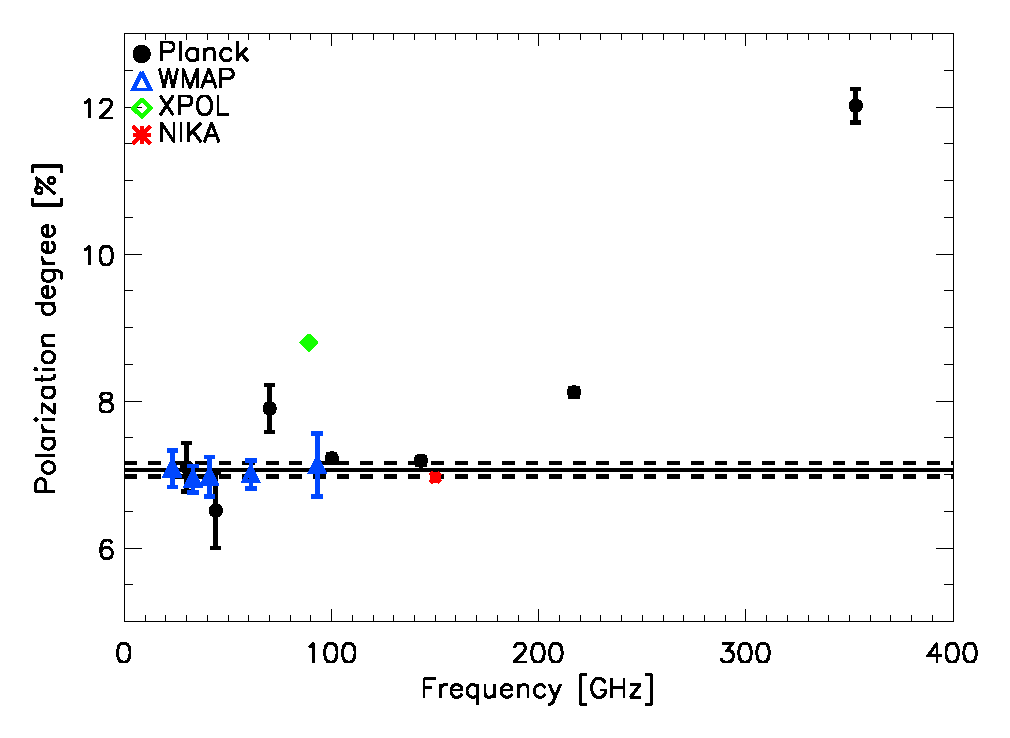
\includegraphics[width=1\linewidth,keepaspectratio]{figures/pdegree_comparison.pdf}}
          { 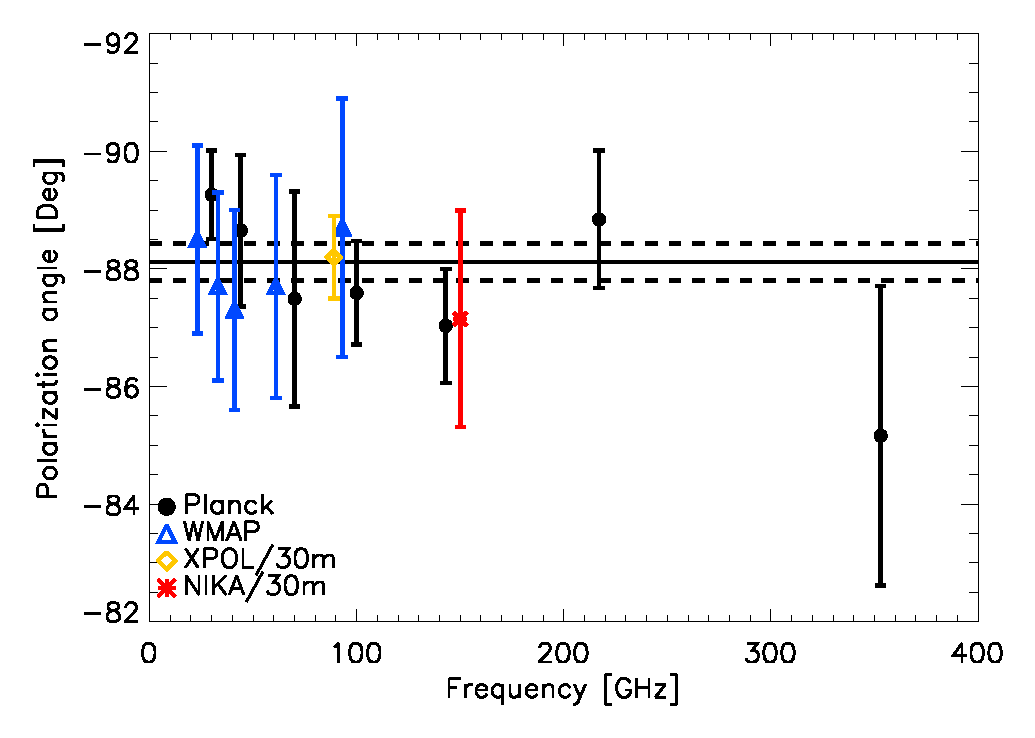
\includegraphics[width=1\linewidth,keepaspectratio]{figures/angle_comparison.pdf}} 
            \caption{{\it Top}: polarization degree as a function of frequency as measured by \Planck\ (black dots), WMAP (blue triangles), XPOL (green diamond), SCUPOL (cyan cross) and \NIKA\ (red crosses). The \NIKA\ value has been estimated by integrating in a radius of $5^{\prime}$ as given by XPOL \citep{aumont2010}. The SCUPOL  values are estimated estimated in a region of 1.4$^\prime$ around the peak of the polarization intensity from the maps in the SCUBA catalogue \citep{scubapol}.
            {\it Bottom}: polarization angles in Galactic coordinates for the same five experiments given above.}
\label{crab_p_angle_comparison}		
  \end{figure}

%\begin{table*}
 % \centering
  %    \begin{tabular}{ccccccccc}
  %    \hline
  %    \hline
  %     Experiments & Frequency & $\psi$ & $p$ & Comments \\ 
  %                                      & [GHz]  & [$^\circ$] & [\%] & \\
  %   \hline
  %   \hline
  %   \NIKA\ &  150 & -87.15 $\pm$ 0.01 (stat) $\pm$ 1.8 (syst) & 6.97$\pm$0.04 & This paper\\
  %  \Planck\ & 143 & -87.03 $\pm$ 0.97 & 7.19 $\pm$ 0.05 & \citep{2015arXiv150702058P} \\
  %   XPOL & 90 & -88.2 $\pm$ 0.7 & 8.8 $\pm$ 0.02 & \citep{aumont2010} \\
  %   \WMAP\ & 94 & -88.7 $\pm$ 2.2 & 7.13 $\pm$ 0.43 & \citep{2011ApJS..192...19W} \\
  %  \hline
  %  \hline   
  %  \end{tabular}
  %  \caption{Polarization angle and degree results obtained by four different experiments. For \NIKA\ and XPOL we estimate the values in five arcmin angular size, which corresponds to the beam of \Planck\ and \WMAP\ at 143 and 94 GHz, respectively.}
  %  \end{table*}

\NIKA\ and XPOL polarization fraction estimates are not consistent. This can be explained by the discrepancy observed in the total intensity as measured by the two instruments, see Fig.~\ref{crab_SED}. A lower total intensity measured produces a higher polarization degree. 


\section{Crab SED}\label{sec:Polarization intensity Spectral Energy Density (SED)}
\subsection{Intensity}
As previously stated observing the Crab nebula is particularly interesting for its angular extension, which is compatible with the typical beam of a CMB experiment, and for its stability across the millimeter wavelengths range. 
Its total intensity emission at millimeter wavelengths (1 and $10^6$ GHz) is mainly due to the synchrotron emission and can be described by a single power law:

\begin{equation}
I_{\nu} = A(\nu / 1 GHz)^{\beta}
\end{equation}\label{eq:sync}
 with spectral index $\beta$ = -0.296$\pm$0.06 \citep{baars1977absolute,macias2010}. At submillimeter wavelengths 10-100 $\mu$m a cold dust component is also observed. Further, the Crab nebula is fading with time at a rate of $\alpha$ = 0.167$\pm$0.015 \% yr$^{-1}$ \citep{aller1985decrease}. 
These observations suggest a low frequency emission produced by particles accelerated by the same magnetic field. The direction of the polarization is thus expected to be constant across frequencies while the polarization degree may vary. 

In order to compare the \NIKA\ results with previous analysis we represent in Fig.~\ref{crab_SED} the intensity flux of the Crab nebula as a function of frequency. The fluxes in the radio domain were taken from \cite{dmitrenko1970absolute} and \cite{1971IzVUZ..14..157V}. We also show microwave and mm wavelengths fluxes from \Archeops\ \citep{macias2007archeops}, \Planck\ \citep{2015arXiv150702058P}, WMAP \citep{2011ApJS..192...19W} and MAMBO \citep{2002A&A...386.1044B}. \NIKA\ intensity flux at 150 GHz is shown in red.
We also represent in the figure the best-fit model to the date computed by $\chi^2$-minimization of observations below 100 GHz. The amplitude and spectral index found are: 

\begin{equation}
 A = 980.6 \pm 0.7  ,\quad \beta = -0.3151 \pm 0.0002. 
 \end{equation}
 For illustration we also show the best fit model found by \cite{macias2010} in a previous analysis. 
Notice that fading is accounted for in the best-fit estimation as well as in the data represented in figure, to ease the interpretation of the plot.
The estimated best-fit model (cyan line) is a bit different w.r.t the previous analysis (green line) mainly due to the addition of recently published results by \Planck\ \citep{2015arXiv150702058P} and  WMAP \citep{2011ApJS..192...19W}. However, the result found at 150 GHz by the \NIKA\ camera agrees in 1 $\sigma$ uncertainty with both models. 
Notice that XPOL intensity is a bit low with respect to what expected by the two power law models. 
 
From the Fig.~\ref{crab_SED} the \Planck\ data at 100, 143, 217 and 353 GHz would suggest an another emission component in the Crab. The break observed around 90 GHz   suggest that another population of electrons contributes to the intensity emission. The results obtained by {\it Archeops}, MAMBO and \NIKA\ do not agree with this conclusion. 
However we estimated the coefficients of the fit in the frequency range 100 $\textless$ $\nu$ $\textless$ 360 GHz and they are: A = 8.6 $\pm$ 0.45 and $\beta$ = -0.71 $\pm$ 0.09. 
\NIKA\ result is in agreement within 2 $\sigma$ with the estimated fit at higher frequencies found using \Planck\ observations.
 Further high angular resolution observations in this frequency range are needed to a better understanding of the emission spectrum. 


\subsection{Polarization}
The total intensity of the Crab nebula has been monitored along decades across a large range of frequency but the amount of polarization observations is really poor.
The recent results provided by \Planck\ \citep{2015arXiv150702058P}, \WMAP\ \citep{2011ApJS..192...19W}, XPOL \citep{aumont2010} allow together with \NIKA\ to trace the polarization intensity SED, see Fig.~\ref{crab_SED_ipol}. The different values measured by \Planck\ are quite different between each other, while the \WMAP\ results are consistent with a power law decreasing with frequency. 
Assuming a power law as described by the Eq.~\ref{eq:sync} we estimate two models represented in blue and black in the figure, which account for only \WMAP\ data and \Planck\ data, respectively.
Accounting for fading the fitted amplitude and spectral indexes $\beta$ are:
\begin{itemize}
\item best fit results using only the WMAP data:
\begin{equation}
A = 78.9\pm7.8 \quad , \quad \beta_p = -0.35\pm0.03;
\end{equation}
\item best fit results using only the \Planck\ data:
\begin{equation}
A = 179.1\pm15.4 \quad , \quad \beta_p = -0.54\pm0.02.
\end{equation}
\end{itemize}

The ``\WMAP'' model seems to be also in agreement with \Planck\ observations at 30, 100 and 353 GHz. 
The \Planck\ data show a variation in the polarized emission with the frequency, which is not consistent with a synchrotron power law model. 

However, \NIKA\ estimated polarization emission at 150 GHz is well consistent with the ``\WMAP'' model and also consistent in 1$\sigma$ with the ``\Planck'' fit. 
The discrepancy observed between ``\Planck'' data evidences the need of high resolution polarization observations of the Crab nebula. 
%By contrast, the \Planck\ data have a significantly steeper spectral index. This model is not consistent neither with the \Planck\ observation at 70 and 353 GHz nor with the \WMAP\ observations except for the point at 61 GHz.
\begin{figure}
  \centering
          { 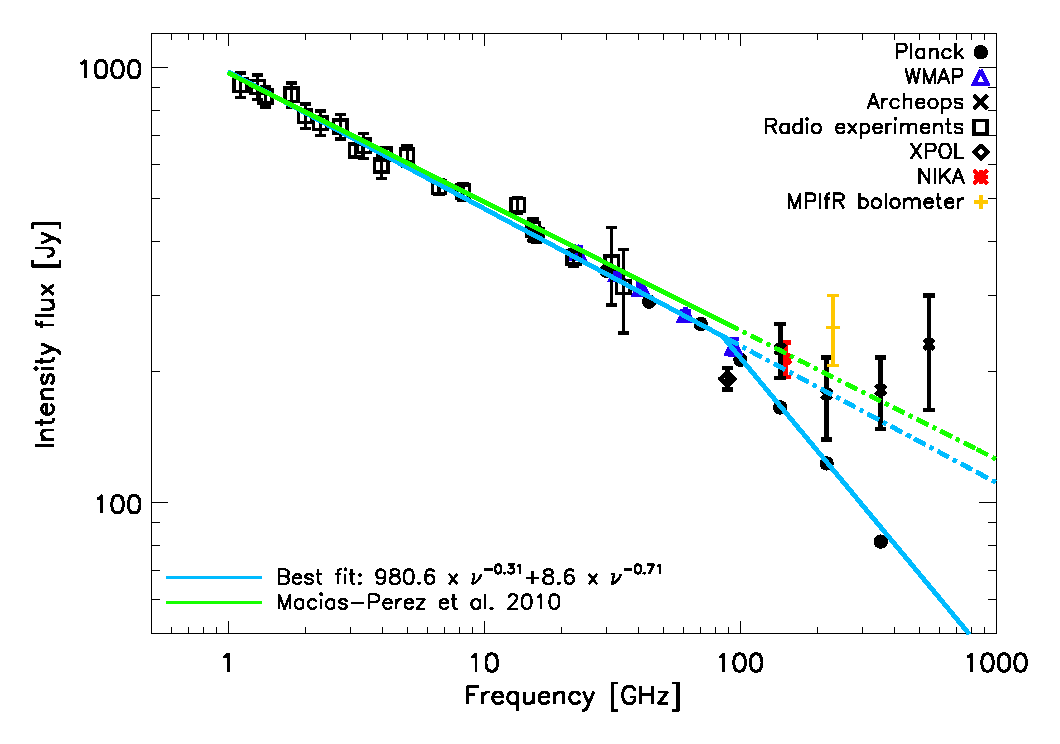
\includegraphics[width=1\linewidth,keepaspectratio]{figures/Crab_SED_i_150.pdf}}
           \caption{Crab nebula total intensity SED. The green line shows the model derived by a previous analysis discussed in \citep{macias2010}. The best-fit obtained by a new analysis is shown in cyan line. Both, the fit and the data account for the fading with the time.}
\label{crab_SED}		
  \end{figure} 

\begin{figure}
  \centering
             { 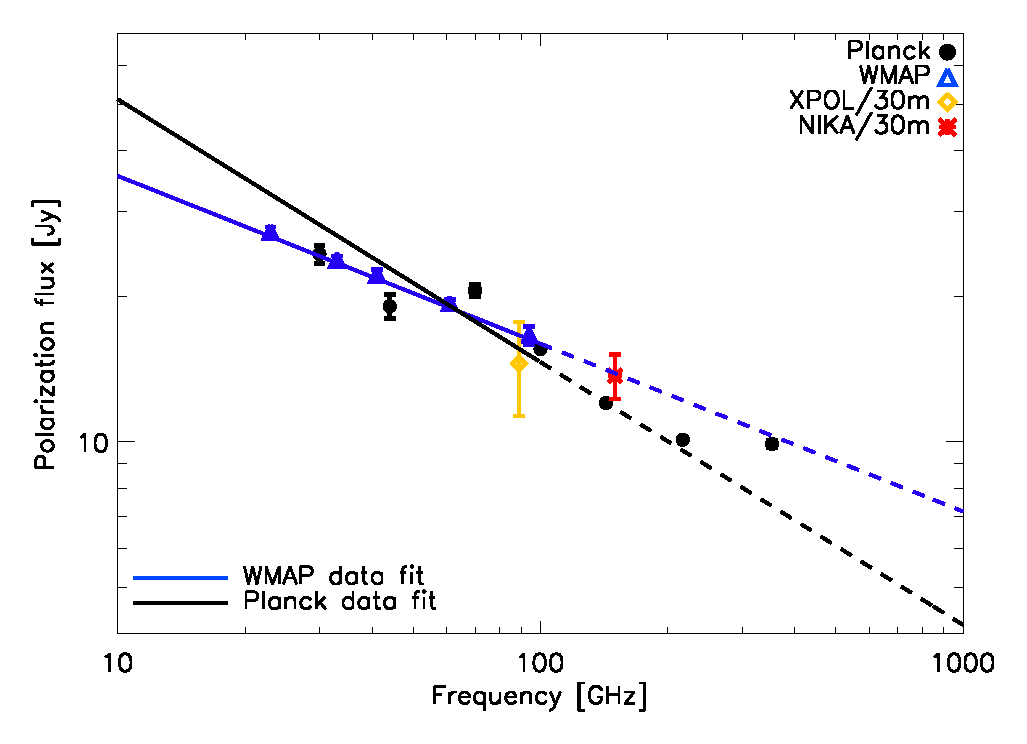
\includegraphics[width=1\linewidth,keepaspectratio]{figures/Crab_SED_ipol.pdf}}
           \caption{Crab nebula polarization intensity SED. The two best-fit models presented have been estimated using only WMAP data (blu line) or \Planck\ data only (black line).}
\label{crab_SED_ipol}		
  \end{figure} 
 \noindent

In order to confirm the spectral index estimated by the ``\WMAP'' model we use the map obtained by SCUPOL at 352 GHz (850 $\mu$m) and the \NIKA\ map, taking only the region observed by SCUPOL, to derive the spectral index:
\begin{equation}
\beta_p = -0.33 \pm 0.01.
\end{equation}
This result is in a very good agreement with what obtained by the ``\WMAP'' model.

%The left panel of Fig.~\ref{crab_beta_ipol} represents the spatial distribution of the spectral index $\beta$ where $I$ $\textgreater$ 3$\sigma$. $\beta$ is obtained as described by the Eq.~\ref{beta_equation} considering the \NIKA\ Stokes $I$ maps of Fig.~\ref{crab_intensity_maps} and accounting for the corresponding frequencies. 

%The right panel of Fig.~\ref{crab_beta_ipol} shows the total intensity map values at 260 GHz as function of the total intensity map observed at 150 GHz. The correlation found between the two frequencies suggests the same physical origin of the emission. 
%The value of the spectral index obtained by the fit is:
%\begin{equation}
%\beta = -0.482 \pm 0.002.
%\end{equation}
%The measured value is different from the expected spectral index from previous observation \citet{baars1977absolute,macias2010}. This difference can be explained by the noise decorrelation used, which is different for the two Stokes $I$ map estimation, that causes filtering effect on the map at 260 GHz.
%The measured spectral index is in agreement with what we observe on the map of the spatial distribution of $\beta$. Indeed, $\beta$ remains approximately constant around -0.45 in the most intense emission region of the source. The contours (red) represent the 150 GHz Stokes $I$ emission map. 

%\begin{figure*}[h!]
  %\centering
  %           { 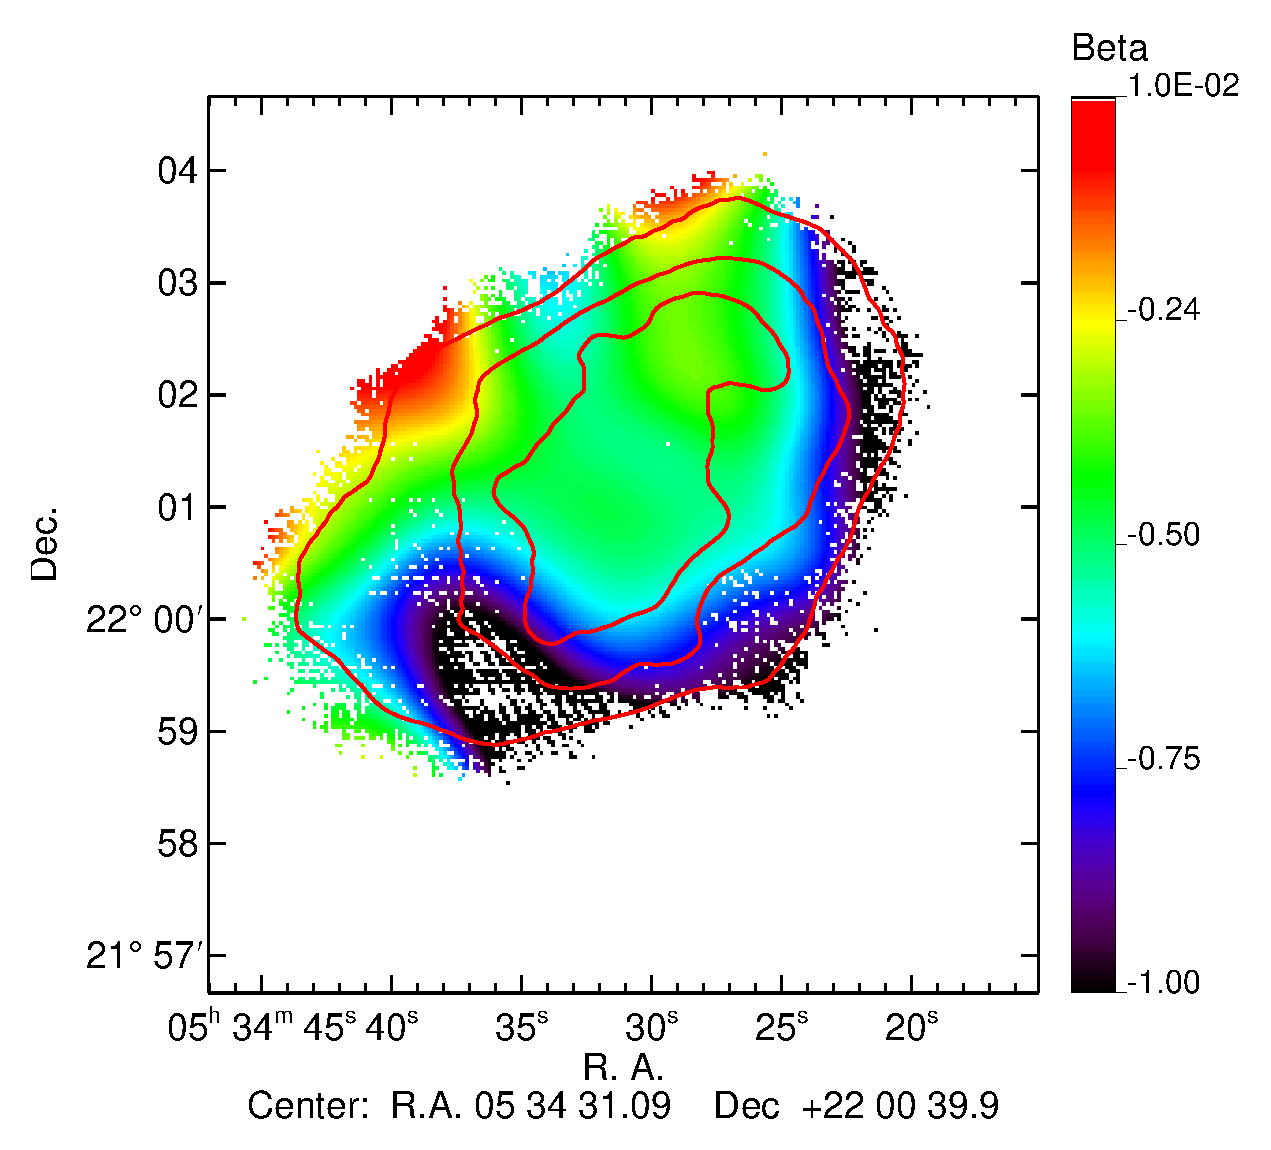
\includegraphics[width=0.4\linewidth,keepaspectratio]{figures/crab_beta_i.pdf}}
  %          { \includegraphics[width=0.5\linewidth,keepaspectratio]{figures/I_1mm_vs_2mm.pdf}}
  %        \caption{Spectral index map (left) obtained using the two NIKA total intensity maps. The correlation between the two maps is shown on the right panel.}
%\label{crab_beta_ipol}		
%  \end{figure*} 
%\subsection{Polarization spectral index}
%In polarization the low S/N observed at 260 GHz prevents us to have a significant detection and to derive the spatial distribution of the spectral index.



\section{Conclusions}\label{sec:conclusions}
The Crab nebula is considered an absolute calibrator for CMB experiments in terms of polarization degree and angle. This absolute calibration is particularly important for the measurement of the CMB polarization B-modes, which are a window towards the physics of the early Universe.

We have reported in this paper first high resolution polarization measurements of the Crab nebula at 150 GHz. These \NIKA\ observations has allowed us to accurately map the spatial distribution of the polarization fraction and angle. 
We find an averaged polarization angle of -87.15$\pm$0.04$\pm$1.8 within a region of 5$^\prime$.
This is consistent with previous measurements from \Planck, \WMAP, and XPOL.
Using the \NIKA\ data in combination with previous observations we have characterized the polarization SED of the Crab nebula. We find that the data are overall consistent with a power law spectrum as expected from synchrotron emission. However, we find some discrepancies between data sets, which requires future mm measurements at high resolution. 

\vspace{0.2cm}
 \begin{acknowledgements}
We would like to thank the IRAM staff for their support during the \NIKA\ campaigns. 
The NIKA dilution cryostat has been designed and built at the Institut N\'eel. 
In particular, we acknowledge the crucial contribution of the Cryogenics Group, and 
in particular Gregory Garde, Henri Rodenas, Jean Paul Leggeri, Philippe Camus. 
This work has been partially funded by the Foundation Nanoscience Grenoble, the LabEx FOCUS ANR-11-LABX-0013 and 
the ANR under the contracts ``MKIDS'', ``NIKA'' and ANR-15-CE31-0017. 
This work has benefited from the support of the European Research Council Advanced Grant ORISTARS 
under the European Union's Seventh Framework Programme (Grant Agreement no. 291294).
We acknowledge fundings from the ENIGMASS French LabEx (R. A. and F. R.), 
the CNES post-doctoral fellowship program (R. A.),  the CNES doctoral fellowship program (A. R.) and 
the FOCUS French LabEx doctoral fellowship program (A. R.).
\end{acknowledgements}


\bibliography{bib_crab.bib}


\end{document}
